%%%%%%%%%%%%%%%%%%%%%%%%%%%%%%%%%%%%%%%%%%%%%%%%%%%%%%%%%%%%%%%%%%%%%%%%%%%%%%%%
\chapter{Αποτελέσματα}

%%%%%%%%%%%%%%%%%%%%%%%%%%%%%%%%%%%%%%%%%%%%%%%%%%%%%%%%%%%%%%%%%%%%%%%%%%%%%%%%
\section{Καταγραφή της Κίνησης}

Ως αποτελέσματα της καταγραφής της κίνησης επιλέχθηκε αρχικά να παρουσιαστεί η ικανότητα καταγραφής του μήκους των τμημάτων του ανθρώπινου σώματος. Στο πείραμα συμμετείχαν δύο δείγματα τα οποία εκτέλεσαν διαφορετικές κινήσεις, όπου για κάθε κίνηση υπολογίστηκε το μέσο μήκος των τμημάτων του σώματος. Αφού συγκεντρώθηκαν τα αποτελέσματα, κατασκευάστηκαν τα αντίστοιχα διαγράμματα που δείχνουν το μέσο μήκος από όλες τις καταγεγραμμένες κινήσεις για κάθε τμήμα μαζί με τις αντίστοιχες τυπικές αποκλίσεις.

\begin{figure}[H]
    \centering
    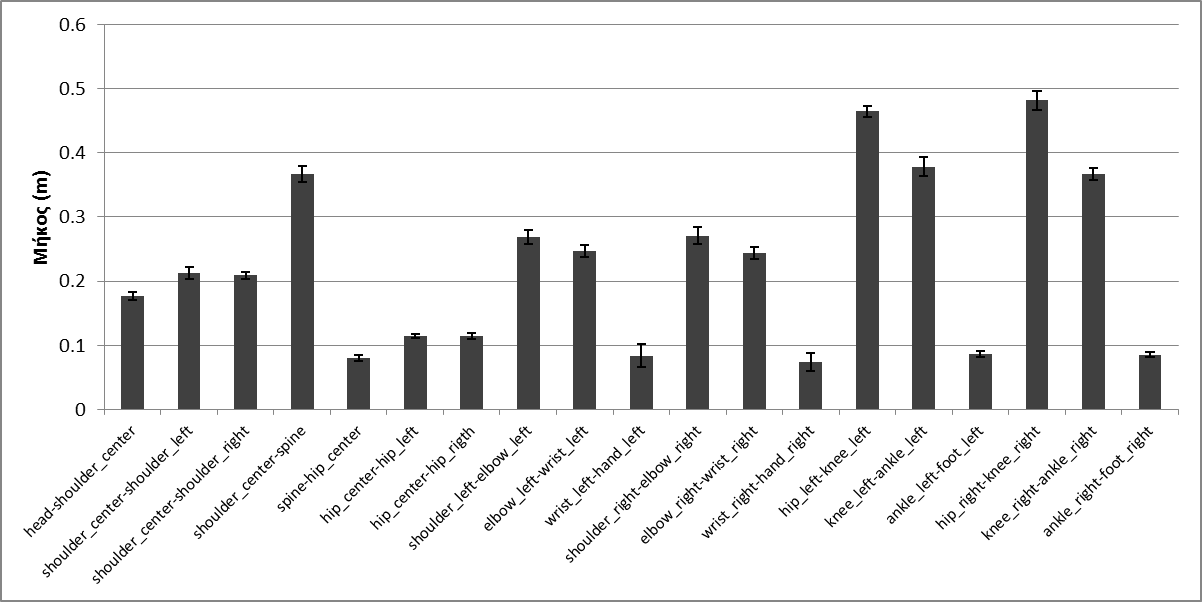
\includegraphics[width=.8\textwidth]{fig/subject01-segments.png}
    \caption{Εκτιμώμενη μέση τιμή σε σύγκριση με την πραγματική τιμή για το μήκος των τμημάτων του σώματος για το πρώτο δείγμα (14 διαφορετικές κινήσεις)}
    \label{fig:subject01-segments}
\end{figure}

Παρατηρούμε ότι οι τυπικές αποκλίσεις είναι μικρές με ελάχιστη για το πρώτο δείγμα στα $std_{min} = 0.0030m$ και με μέγιστη τιμή στα $std_{max} = 0.0182m$ \ref{fig:subject01-segments}. Όσον αφορά το δεύτερο δείγμα οι αντίστοιχες τυπικές αποκλίσεις είναι $std_{min} = 0.0.0019m$, $std_{max} = 0.0146m$ αντίστοιχα \ref{fig:subject02-segments}. Επίσης και για τα δυο δείγματα παρουσιάζονται τα πραγματικά μήκη των τμημάτων του σώματος με σφάλμα μετρήσεων $\pm 1cm$.

\begin{figure}[H]
    \centering
    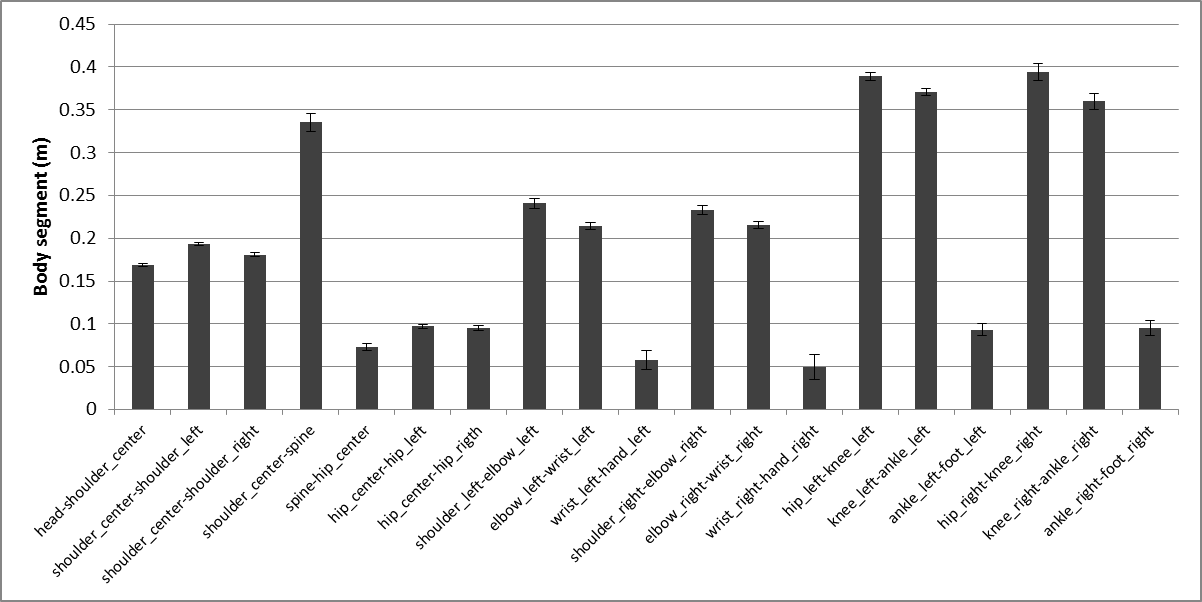
\includegraphics[width=.8\textwidth]{fig/subject02-segments.png}
    \caption{Εκτιμώμενη μέση τιμή σε σύγκριση με την πραγματική τιμή για το μήκος των τμημάτων του σώματος για το δεύτερο δείγμα (5 κινήσεις)}
    \label{fig:subject02-segments}
\end{figure}

\begin{equation}
    \begin{gathered}
        \text{Πρόβλεψη} \\
        \hat{p}_{t} = p_{t-1} + u_{t}, \quad u_{t} = \frac{p_{t-1} - p_{t-2}}{t_{t-1} - t_{t-2}} \\
        \hat{P} = P_{t-1} + Q \\[.5cm]
        \text{Διόρθωση} \\
        Κ = \frac{\hat{P}}{\hat{P} + R}\\
        p_{t} = \hat{p}_{t} + K \cdot (p_{t} - \hat{p}_{t}) \\
        P_{t} = (1 - K) \cdot \hat{P}
    \end{gathered}
    \label{equ:kalman-predict-update}
\end{equation}

Ως δεύτερη σύγκριση του συστήματος, καταγράφτηκε μια κίνηση χωρίς την χρήση κάποιου φίλτρου και στην συνέχεια καταγράφτηκε μια όμοια κίνηση με χρήση φίλτρου και ως παράμετροι επιλέχθηκαν οι τιμές για δυνατό φιλτράρισμα από την εικόνα \ref{tab:filter-parameters}. Επίσης έγινε μια απλή υλοποίηση ενός φίλτρου \eng{Kalman} με βάση την αναδρομική σχέση \ref{equ:kalman-predict-update} και επιλέχθηκαν τιμές για τα $R = 0.05,\; Q = 0.05$. Στην εικόνα \ref{fig:no-filter-filter-kalman} στην αριστερή στήλη βρίσκονται οι συντεταγμένες του δεξιού χεριού χωρίς την χρήση κάποιου φίλτρου, ενώ στην δεξιά στήλη με χρήση του δυνατού φίλτρου. Με διακεκομμένες γραμμές φαίνεται η απόκριση του φίλτρου \eng{Kalman}. Στην περίπτωση που επιλέξουμε να χρησιμοποιήσουμε δυνατό φίλτρο δεν διακρίνεται βελτιώση αν χρησιμοποιήσουμε το φίλτρου \eng{Kalman}, όπως έχει υλοποιηθεί. Φαίνεται όμως η ανάγκη για εξομάλυνση, οπότε απλά φίλτρα που φιλτράρουν τις απότομες μεταβολές βελτιώνουν πολύ το αποτέλεσμα.

%\begin{center}
%    \begin{tabular}{cc}
%        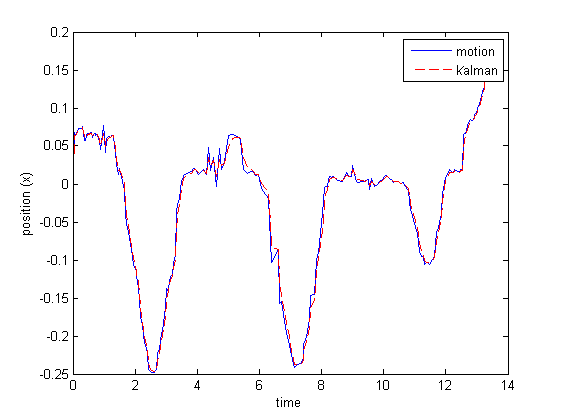
\includegraphics[width=.5\textwidth, height = 0.22\textheight, keepaspectratio]{fig/filter0-x.png} & 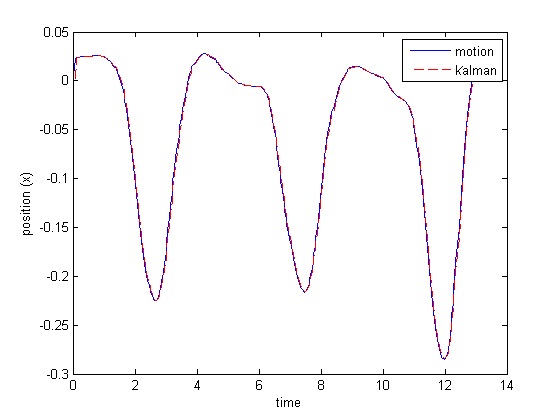
\includegraphics[width=.5\textwidth, height = 0.22\textheight, keepaspectratio]{fig/filter3-x.png}\\
%        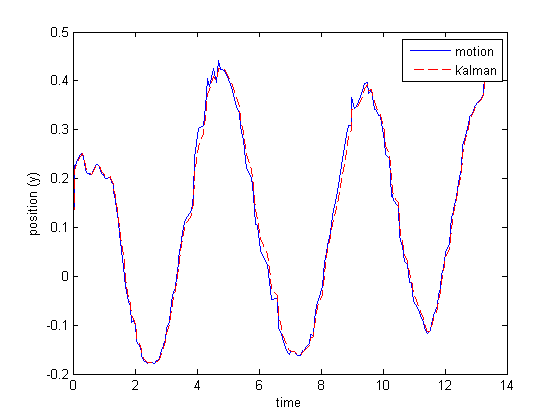
\includegraphics[width=.5\textwidth, height = 0.22\textheight, keepaspectratio]{fig/filter0-y.png} & 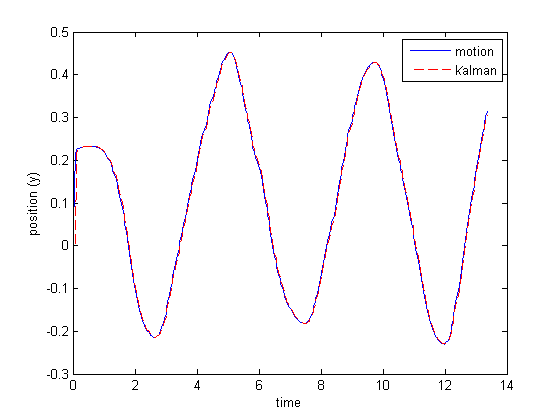
\includegraphics[width=.5\textwidth, height = 0.22\textheight, keepaspectratio]{fig/filter3-y.png}\\
%        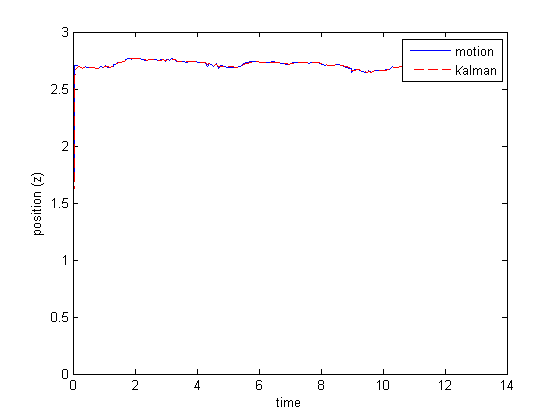
\includegraphics[width=.5\textwidth, height = 0.22\textheight, keepaspectratio]{fig/filter0-z.png} & 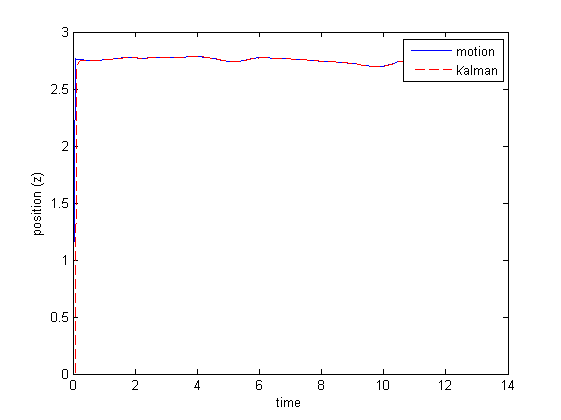
\includegraphics[width=.5\textwidth, height = 0.22\textheight, keepaspectratio]{fig/filter3-z.png}\\
%        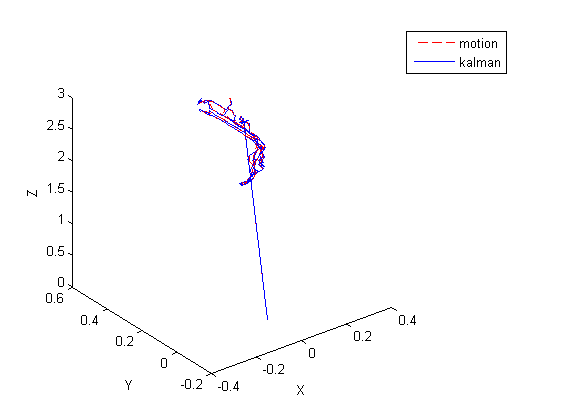
\includegraphics[width=.5\textwidth, height = 0.22\textheight, keepaspectratio]{fig/filter0-xyz.png} & 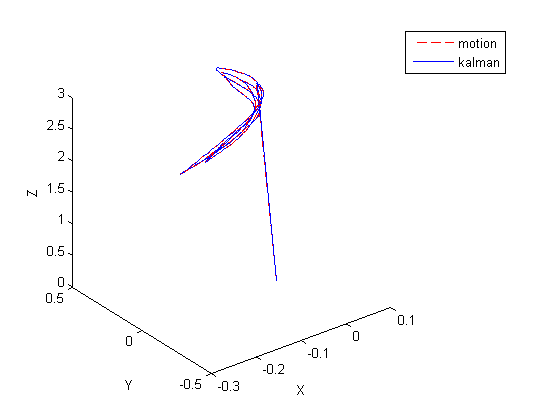
\includegraphics[width=.5\textwidth, height = 0.22\textheight, keepaspectratio]{fig/filter3-xyz.png}
%    \end{tabular}
%    \captionof{table}{Συντεταγμένες του δεξιού χεριού στις επιμέρους συνιστώσες (\eng{x, y, z, xyz}) χωρίς φιλτράρισμα (αριστερή στήλη) και με φιλτράρισμα (δεξιά στήλη) με βάση την υλοποίηση μας. Σύγκριση και στις δυο περιπτώσεις με το φίλτρο \eng{Kalman}}
%    \label{tab:no-filter-filter-kalman}
%\end{center}

\begin{figure}[H]
    %\captionsetup[subfigure]{position=b}
    \centering
    \begin{subfigure}[t]{.48\textwidth}
        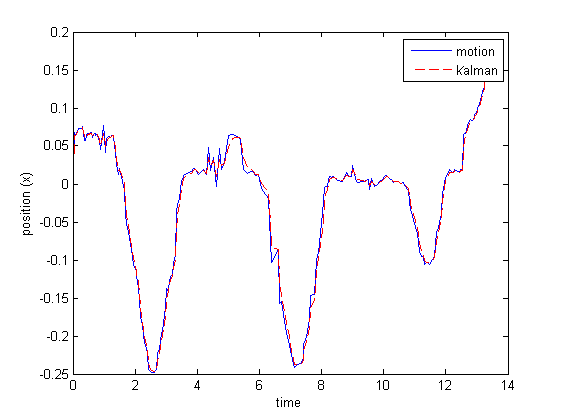
\includegraphics[width=\textwidth, keepaspectratio]{fig/filter0-x.png}
        \caption{Συντεταγμένη στον \eng{x} άξονα χωρίς φιλτράρισμα}
        \label{fig:filter0-x}
    \end{subfigure}
    \begin{subfigure}[t]{.48\textwidth}
        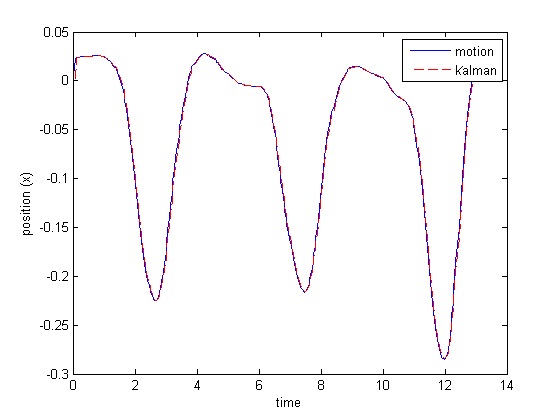
\includegraphics[width=\textwidth, keepaspectratio]{fig/filter3-x.png}
        \caption{Συντεταγμένη στον \eng{x} άξονα με φιλτράρισμα}
        \label{fig:filter3-x}
    \end{subfigure}

    \centering
    \begin{subfigure}[t]{.48\textwidth}
        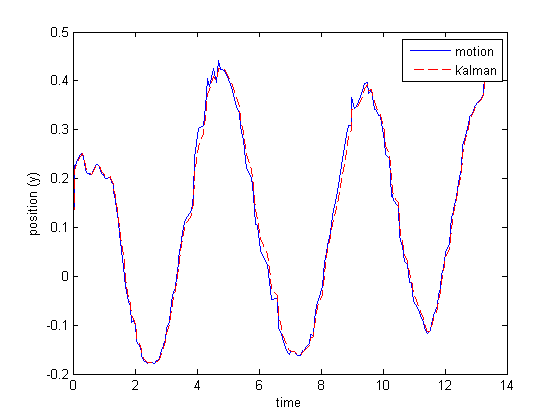
\includegraphics[width=\textwidth, keepaspectratio]{fig/filter0-y.png}
        \caption{Συντεταγμένη στον \eng{y} άξονα χωρίς φιλτράρισμα}
        \label{fig:filter0-y}
    \end{subfigure}
    \begin{subfigure}[t]{.48\textwidth}
        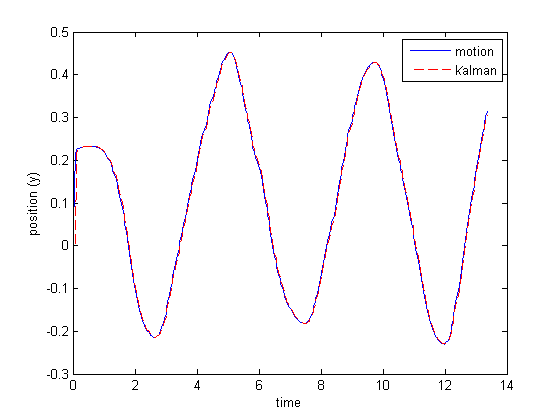
\includegraphics[width=\textwidth, keepaspectratio]{fig/filter3-y.png}
        \caption{Συντεταγμένη στον \eng{y} άξονα με φιλτράρισμα}
        \label{fig:filter3-y}
    \end{subfigure}

    \centering
    \begin{subfigure}[t]{.48\textwidth}
        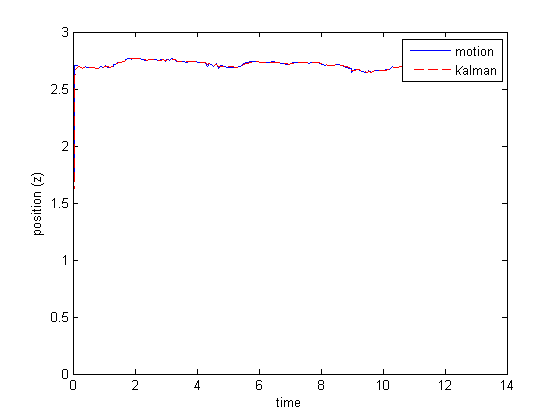
\includegraphics[width=\textwidth, keepaspectratio]{fig/filter0-z.png}
        \caption{Συντεταγμένη στον \eng{z} άξονα χωρίς φιλτράρισμα}
        \label{fig:filter0-z}
    \end{subfigure}
    \begin{subfigure}[t]{.48\textwidth}
        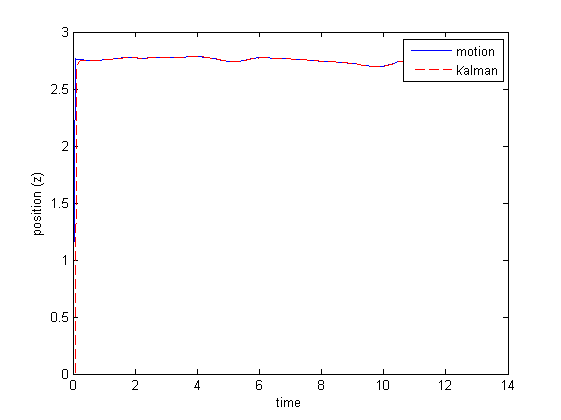
\includegraphics[width=\textwidth, keepaspectratio]{fig/filter3-z.png}
        \caption{Συντεταγμένη στον \eng{z} άξονα με φιλτράρισμα}
        \label{fig:filter3-z}
    \end{subfigure}
    \caption{Συντεταγμένες του δεξιού χεριού στις επιμέρους συνιστώσες (\eng{x, y, z}) χωρίς φιλτράρισμα (αριστερή στήλη) και με φιλτράρισμα (δεξιά στήλη) με βάση την υλοποίηση μας. Σύγκριση και στις δυο περιπτώσεις με το φίλτρο \eng{Kalman}}
    \label{fig:no-filter-filter-kalman}
\end{figure}

%%%%%%%%%%%%%%%%%%%%%%%%%%%%%%%%%%%%%%%%%%%%%%%%%%%%%%%%%%%%%%%%%%%%%%%%%%%%%%%%
\section{Αντίστροφη Κινηματική}

\begin{figure}[H]
    \centering
    \begin{subfigure}[t]{.48\textwidth}
        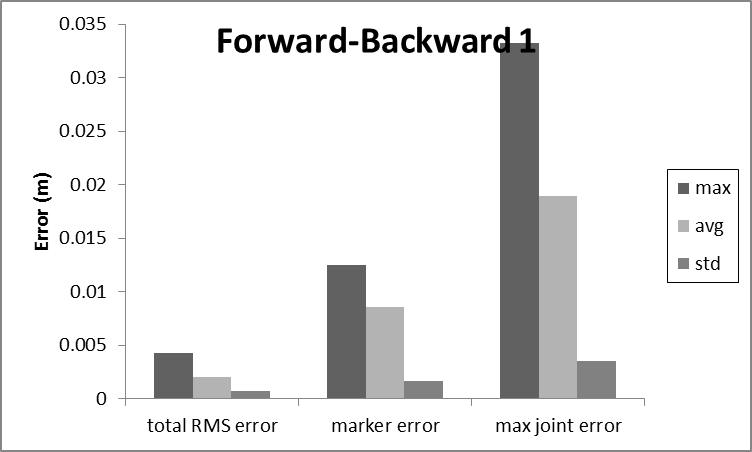
\includegraphics[width=\textwidth, keepaspectratio]{fig/ik-reg1.png}
        \caption{Κίνηση μπροστά-πίσω}
        \label{fig:forth-back1}
    \end{subfigure}
    \begin{subfigure}[t]{.48\textwidth}
        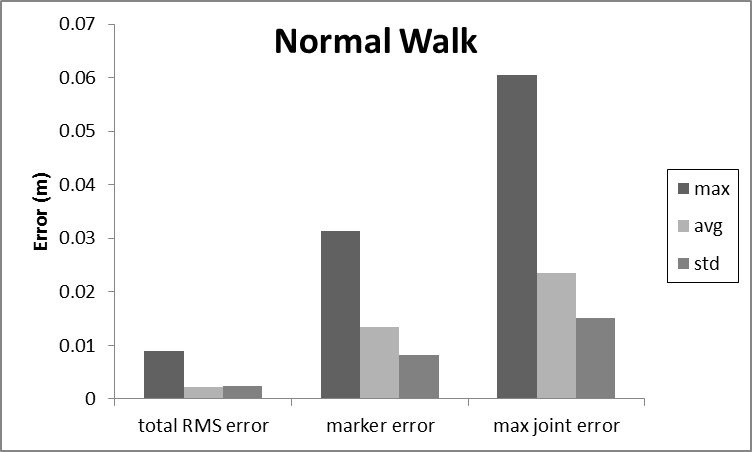
\includegraphics[width=\textwidth, keepaspectratio]{fig/ik-reg2.png}
        \caption{Κίνηση μπροστά-πίσω}
        \label{fig:forth-back2}
    \end{subfigure}

    \begin{subfigure}[t]{.48\textwidth}
        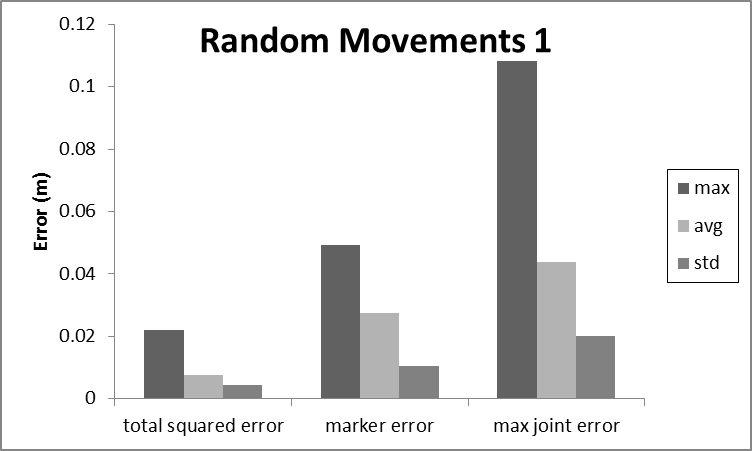
\includegraphics[width=\textwidth, keepaspectratio]{fig/ik-reg3.png}
        \caption{Τυχαία κίνηση}
        \label{fig:random-walk1}
    \end{subfigure}
    \begin{subfigure}[t]{.48\textwidth}
        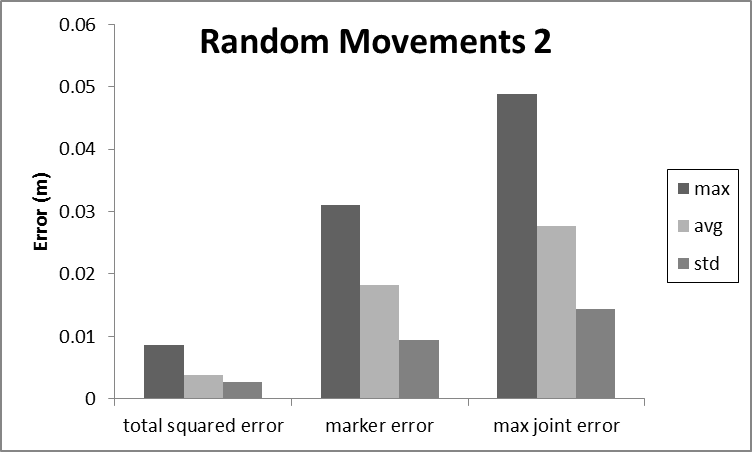
\includegraphics[width=\textwidth, keepaspectratio]{fig/ik-reg4.png}
        \caption{Τυχαία κίνηση}
        \label{fig:random-walk1}
    \end{subfigure}

    \begin{subfigure}[t]{.48\textwidth}
        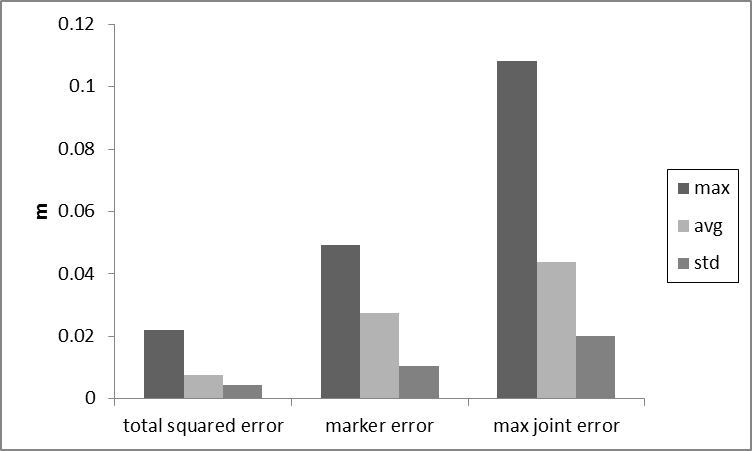
\includegraphics[width=\textwidth, keepaspectratio]{fig/ik-reg5.png}
        \caption{Κανονική βάδιση}
        \label{fig:noraml-walk}
    \end{subfigure}
    \begin{subfigure}[t]{.48\textwidth}
        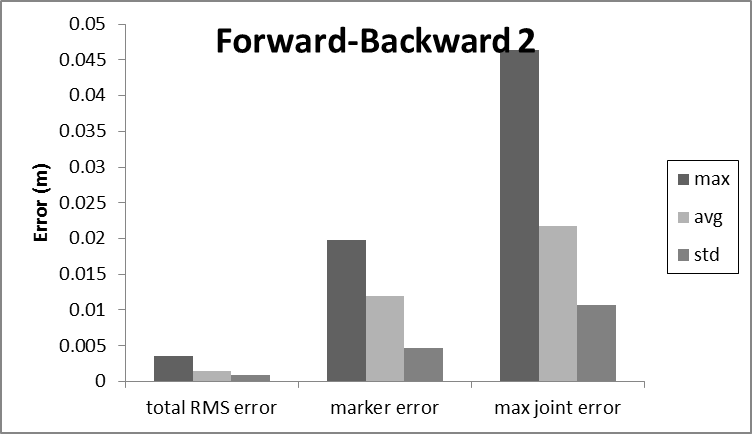
\includegraphics[width=\textwidth, keepaspectratio]{fig/ik-reg6.png}
        \caption{Εμπρόσθια προέκταση του ποδιού}
        \label{fig:knee-hip-extension}
    \end{subfigure}
    \caption{Τα τρία είδη σφαλμάτων της αντίστροφης κινηματικής για τις έξι διαφορετικές κινήσεις. Για τα τρία σφάλματα παρουσιάζονται η μέγιστη τιμή, η μέση τιμή και η τυπική απόκλιση που υπολογίστηκε με βάση την χρονοσειρά των σφαλμάτων}
    \label{fig:ik-error-regions}
\end{figure}

Για να υπάρξουν σωστά αποτελέσματα κατά την αντίστροφη κινηματική είναι αναγκαία η διαδικασία της κανονικοποίησης, ώστε το γενικό μοντέλο να πάρει τις διαστάσεις του δείγματος, οπότε η διαδικασία της κανονικοποίησης θεωρείται δεδομένη κάθε φορά. Αυτό που μπορούμε να εκθέσουμε ως αποτέλεσμα της διαδικασίας είναι τα σφάλματα της αντίστροφης κινηματικής. Για το πείραμα εκτελέστηκε η αντίστροφη κινηματική για 6 διαφορετικές κινήσεις \ref{fig:ik-error-regions} του ίδιου δείγματος και καταγράφηκε το συνολικό τετραγωνικό σφάλμα (\eng{total square error}), το σφάλμα λόγω ενδείξεων (\eng{marker error}) και το μέγιστο σφάλμα από όλες τις αρθρώσεις (\eng{max joint error}). Το συνολικό αθροιστικό σφάλμα λαμβάνεται ως το σφάλμα που οφείλεται στην διαφορά των συντεταγμένων του μοντέλου και της πειραματικής κίνησης. Το σφάλμα λόγω ενδείξεων υπολογίζεται με βάση την Ευκλείδεια απόσταση των ενδείξεων του μοντέλου και των αντίστοιχων πειραματικών. Όσον αφορά το μέγιστο σφάλμα άρθρωσης αφορά την άρθρωση που συνεισφέρει περισσότερο στο σφάλμα. Τα τρία αυτά σφάλματα ήταν διαθέσιμα για κάθε χρονική στιγμή που υπολογίζονταν η αντίστροφη κινηματική. Ως εκ τούτο για κάθε ένα από αυτά τα σφάλματα υπολογίστηκε η μέση τιμή, η τυπική απόκλιση και η μέγιστη τιμή από όλες τις χρονικές στιγμές για κάθε κίνηση ξεχωριστά. Με βάση την βιβλιογραφία αναφέρεται ότι το συνολικό τετραγωνικό σφάλμα πρέπει να είναι μικρότερο του $0.01cm$ και για το σφάλμα λόγω ενδείξεων να κυμαίνεται στα όρια $[0.02-0.04cm]$, ώστε να έχουμε ικανοποιητική ανοχή στα αποτέλεσμα της αντίστροφης κινηματικής.

%\begin{center}
%    \begin{tabular}{cc}
%        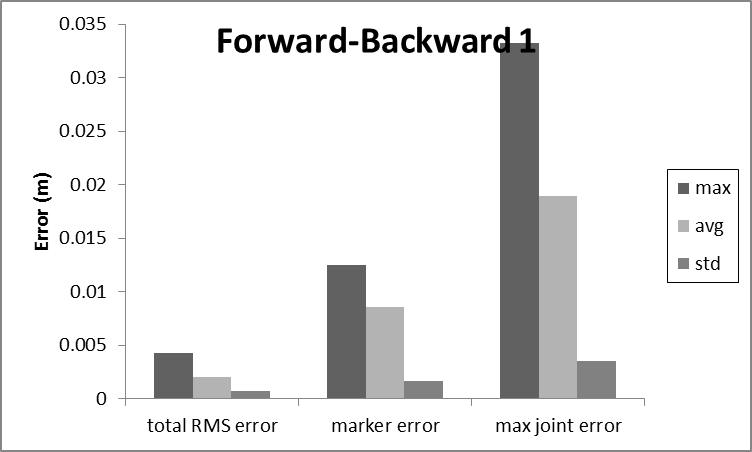
\includegraphics[width=.48\textwidth, keepaspectratio]{fig/ik-reg1.png} & 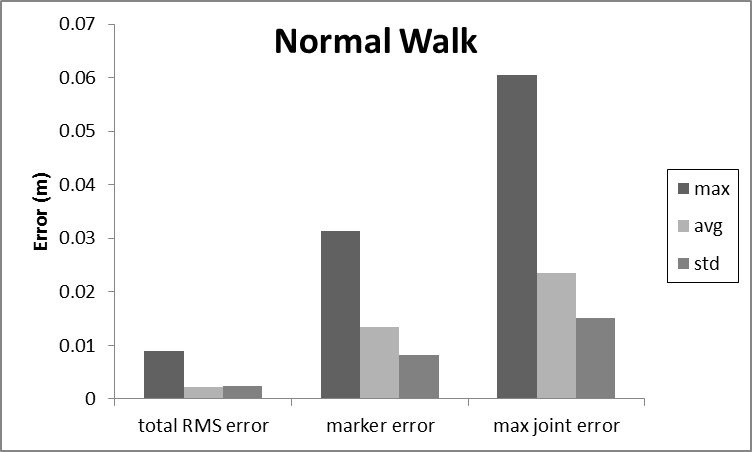
\includegraphics[width=.48\textwidth, keepaspectratio]{fig/ik-reg2.png}\\[3pt]
%        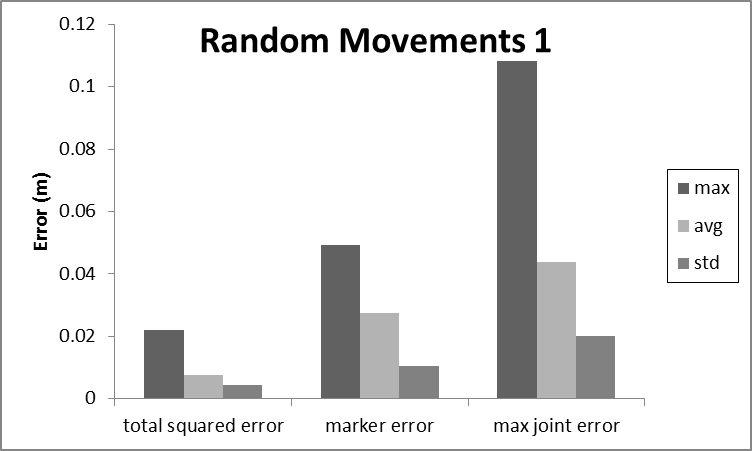
\includegraphics[width=.48\textwidth, keepaspectratio]{fig/ik-reg3.png} & 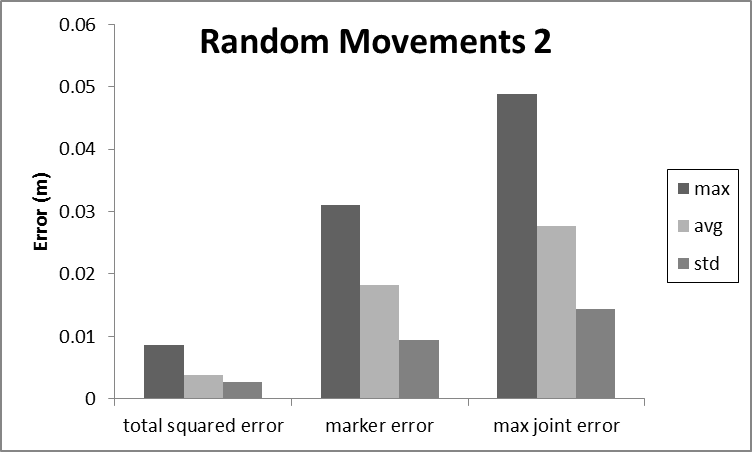
\includegraphics[width=.48\textwidth, keepaspectratio]{fig/ik-reg4.png}\\[3pt]
%        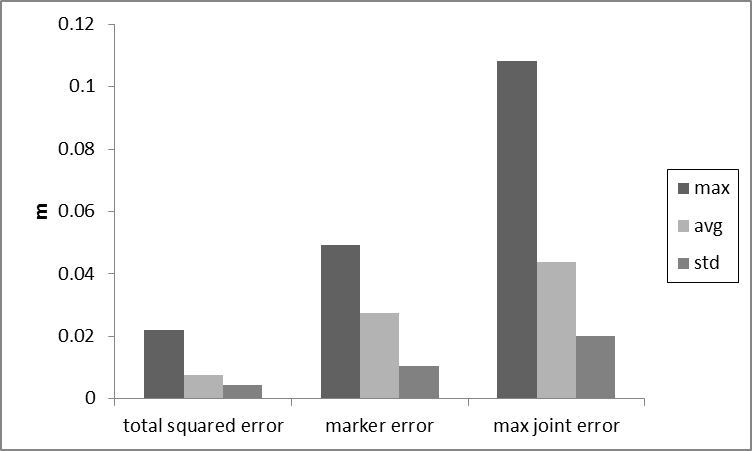
\includegraphics[width=.48\textwidth, keepaspectratio]{fig/ik-reg5.png} & 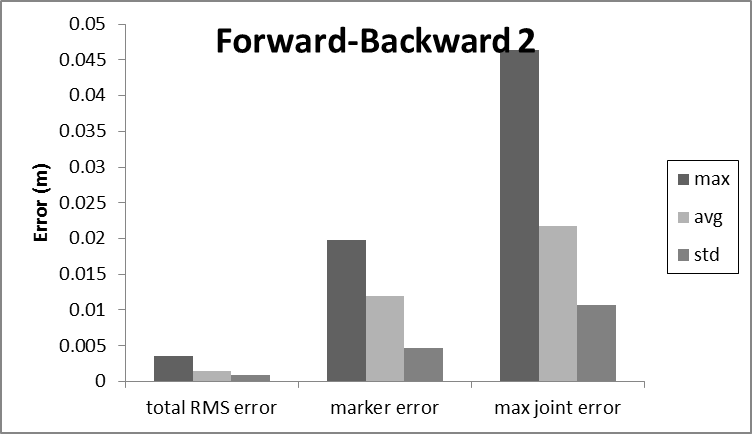
\includegraphics[width=.48\textwidth, keepaspectratio]{fig/ik-reg6.png}
%    \end{tabular}
%    \captionof{table}{Τα τρία είδη σφαλμάτων της αντίστροφης κινηματικής για τις έξι διαφορετικές κινήσεις. Για τα τρία σφάλματα παρουσιάζονται η μέγιστη τιμή, η μέση τιμή και η τυπική απόκλιση που υπολογίστηκε με βάση την χρονοσειρά των σφαλμάτων.}
%    \label{tab:ik-error-regions}
%\end{center}

\begin{figure}[H]
    \centering
    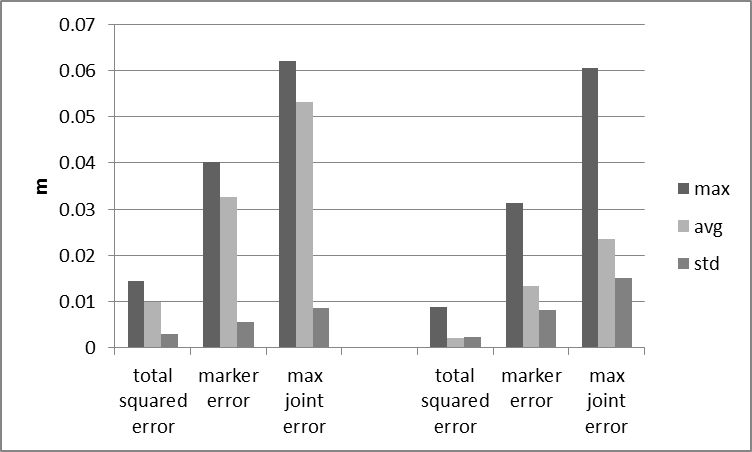
\includegraphics[width=0.8\textwidth, keepaspectratio]{fig/ik-no-scale-with-scale.png}
    \caption{Σύγκριση της βελτίωσης των σφαλμάτων της αντίστροφης κινηματικής με ή χωρίς την εκτέλεση της κανονικοποίησης}
    \label{fig:ik-no-scale-with-scale}
\end{figure}

Στην εικόνα \ref{fig:ik-no-scale-with-scale} έγινε σύγκριση της αποτελεσματικότητας της διαδικασία κανονικοποίησης στο αποτέλεσμα της αντίστροφης κινηματικής. Η πρώτη τριάδα των μετρήσεων αφορά τα σφάλματα της αντίστροφης κινηματικής χωρίς την διεξαγωγή κανονικοποίησης, ενώ η δεύτερη τριάδα με διεξαγωγή της κανονικοποίησης. Παρατηρείται μεγάλη βελτίωση των σφαλμάτων και ιδιαίτερα στα σφάλματα μέσης τιμής. Ωστόσο δεν παρατηρείται σημαντική βελτίωση στα σφάλματα της μέγιστης τιμής σφάλματος της άρθρωσης. Δηλαδή υπάρχουν κάποιες αρθρώσεις που δίνουν μεγάλο σφάλμα, αλλά γενικά έχουμε βελτίωση ως προς το μέσο όρο των αρθρώσεων.

%%%%%%%%%%%%%%%%%%%%%%%%%%%%%%%%%%%%%%%%%%%%%%%%%%%%%%%%%%%%%%%%%%%%%%%%%%%%%%%%
\section{Αντίστροφη Δυναμική}

\begin{figure}[H]
    \centering
    \begin{subfigure}[t]{.48\textwidth}
        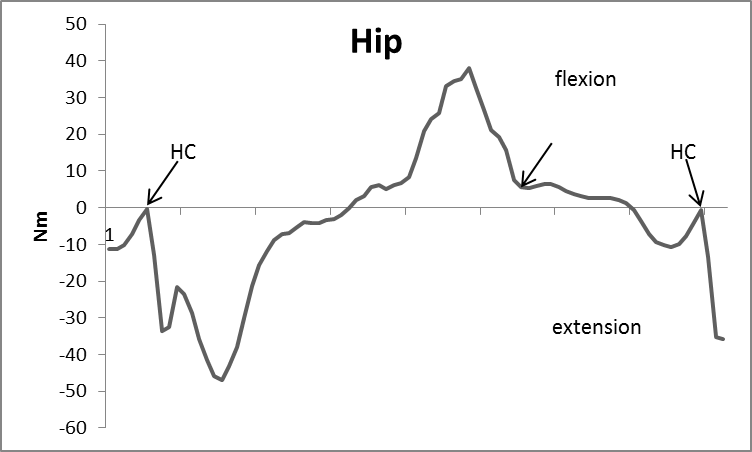
\includegraphics[width=\textwidth, keepaspectratio]{fig/id-hip.png}
        \caption{Ροπή στο γοφό συναρτήσει για έναν κύκλο βάδισης (πειραματικά)}
        \label{fig:hip-moment}
    \end{subfigure}
    \begin{subfigure}[t]{.48\textwidth}
        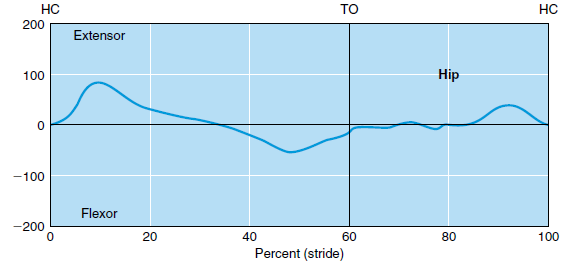
\includegraphics[width=\textwidth, keepaspectratio]{fig/id-hip-ref.png}
        \caption{Ροπή του γοφό συναρτήσει για έναν κύκλο βάδισης (βιβλιογραφία)}
        \label{fig:hip-moment-ref}
    \end{subfigure}

    \centering
    \begin{subfigure}[t]{.48\textwidth}
        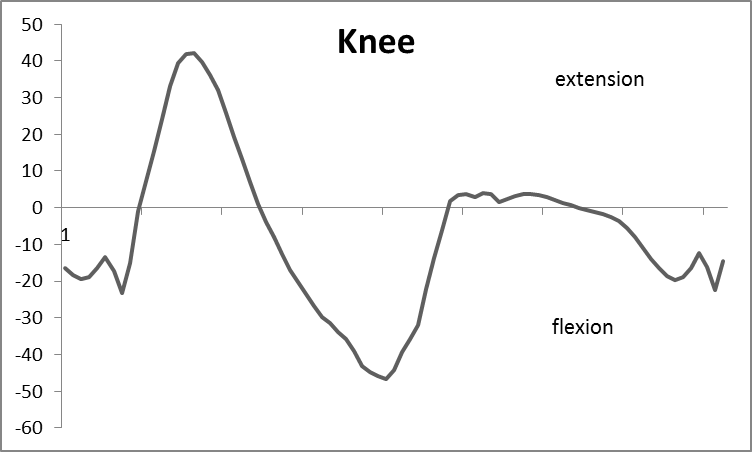
\includegraphics[width=\textwidth, keepaspectratio]{fig/id-knee.png}
        \caption{Ροπή στο γόνατο συναρτήσει για έναν κύκλο βάδισης (πειραματικά)}
        \label{fig:knee-moment}
    \end{subfigure}
    \begin{subfigure}[t]{.48\textwidth}
        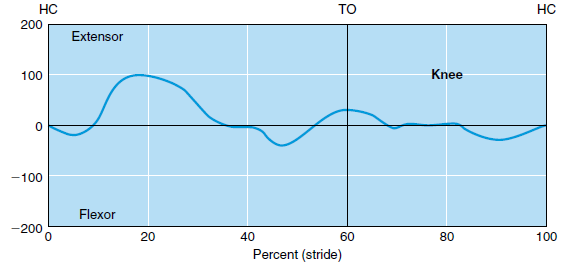
\includegraphics[width=\textwidth, keepaspectratio]{fig/id-knee-ref.png}
        \caption{Ροπή στο γονάτο συναρτήσει για έναν κύκλο βάδισης (βιβλιογραφία)}
        \label{fig:knee-moment-ref}
    \end{subfigure}

    \centering
    \begin{subfigure}[t]{.48\textwidth}
        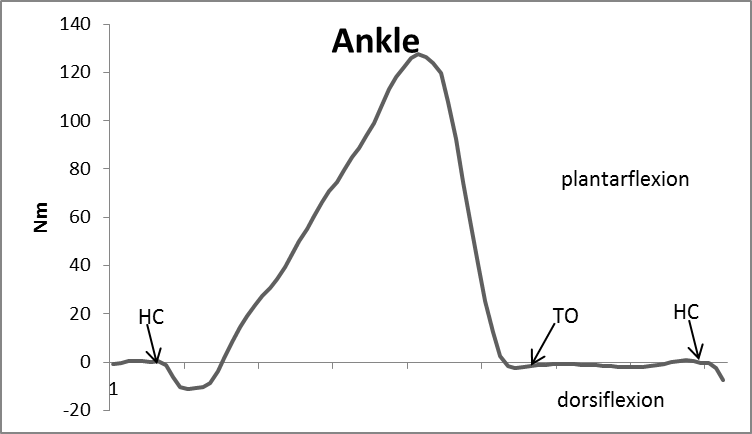
\includegraphics[width=\textwidth, keepaspectratio]{fig/id-ankle.png}
        \caption{Ροπή στο αστράγαλο συναρτήσει για έναν κύκλο βάδισης (πειραματικά)}
        \label{fig:ankle-moment}
    \end{subfigure}
    \begin{subfigure}[t]{.48\textwidth}
        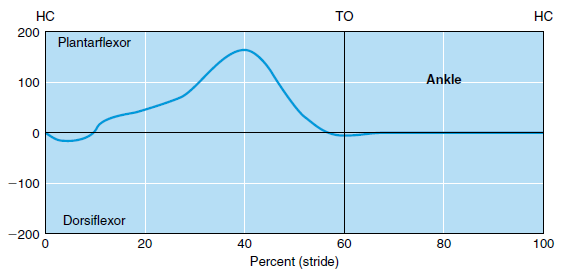
\includegraphics[width=\textwidth, keepaspectratio]{fig/id-ankle-ref.png}
        \caption{Ροπή στον αστράγαλο συναρτήσει για έναν κύκλο βάδισης (βιβλιογραφία)}
        \label{fig:ankle-moment-ref}
    \end{subfigure}
    \caption{Σύγκριση εκτιμώμενων ροπών και των αντίστοιχων ροπών με βάση την βιβλιογραφία \cite{whittlesey} για ένα κύκλο βάδισης}
    \label{fig:id-hip-knee-ankle-moments}
\end{figure}

Με την αντίστροφη δυναμική έχουμε στην διάθεση μας τις ροπές που ασκούνται στις αρθρώσεις κάθε χρονική στιγμή. Λόγω της δυσκολίας υπολογισμού των εξωτερικών δυνάμεων, χρησιμοποιήθηκαν δεδομένα βάδισης και καταγεγραμμένη αντίδραση εδάφους που βρέθηκε στο διαδίκτυο, ώστε να επιβεβαιωθεί η ισχύς της ανάλυσης. Στην μελέτη των δυνάμεων, παρουσιάζονται οι ροπές του γοφού, του γονάτου και του αστράγαλου σε ένα κύκλο βάδισης και συγκρίνονται με την βιβλιογραφία \cite{whittlesey}. Στην εικόνα \ref{fig:id-hip-knee-ankle-moments} αριστερά βρίσκονται οι πειραματικές ροπές για έναν κύκλο βάδισης και δεξιά τα αντίστοιχα με βάση τη βιβλιογραφία. Όσον αφορά τις κυματομορφές \ref{fig:hip-moment} και \ref{fig:ankle-moment} παρουσιάζονται ανεστραμμένα  γιατί έχουμε θεωρήσει διαφορετικές φορές στους βαθμούς ελευθερίας, ωστόσο τα αποτελέσματα μας συμβαδίζουν με εκείνα της βιβλιογραφίας αν λάβουμε υπόψιν τις ενδείξεις πάνω στα διαγράμματα. Επίσης παρατηρείται απόκλιση στις μέγιστες και ελάχιστες τιμές με εκείνες τις βιβλιογραφίας, επειδή για τα αποτελέσματα της βιβλιογραφίας χρησιμοποιείται το μοντέλου όλου του σώματος, ενώ στα δικά μας χρησιμοποιείται μόνο το κάτω μέρος με αποτέλεσμα να ζυγίζει λιγότερο και η απαιτούμενη ροπή στις αρθρώσεις να είναι μικρότερη. Ωστόσο ποιοτικά τα αποτελέσματα μας συμβαδίζουν με τα προβλεπόμενα.

%\begin{center}
%    \begin{tabular}{cc}
%        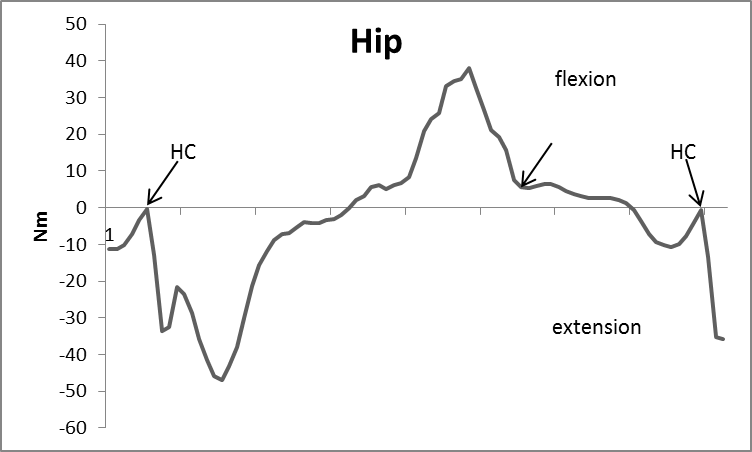
\includegraphics[width=.48\textwidth, keepaspectratio]{fig/id-hip.png} & 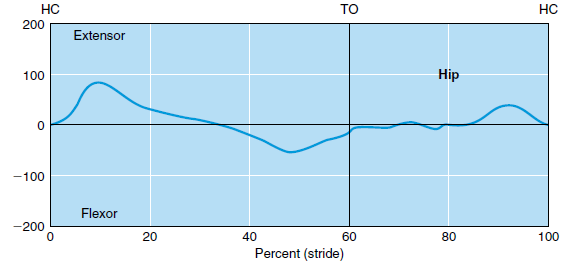
\includegraphics[width=.48\textwidth, keepaspectratio]{fig/id-hip-ref.png}\\[3pt]
%        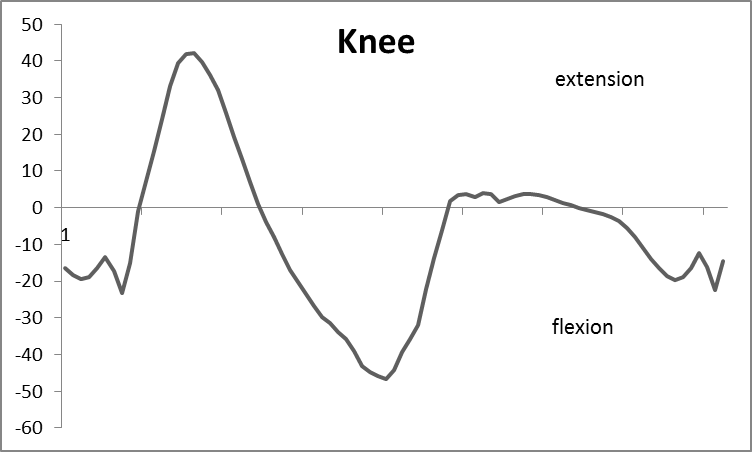
\includegraphics[width=.48\textwidth, keepaspectratio]{fig/id-knee.png} & 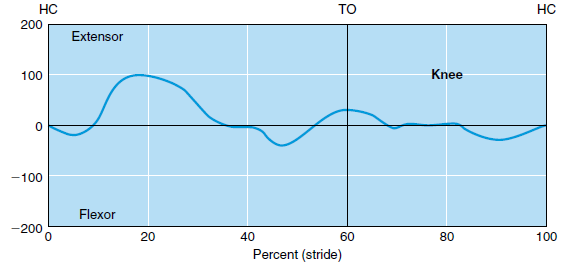
\includegraphics[width=.48\textwidth, keepaspectratio]{fig/id-knee-ref.png}\\[3pt]
%        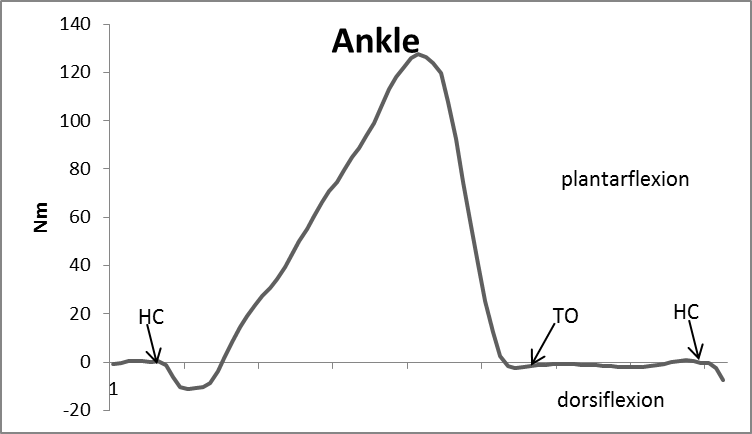
\includegraphics[width=.48\textwidth, keepaspectratio]{fig/id-ankle.png} & 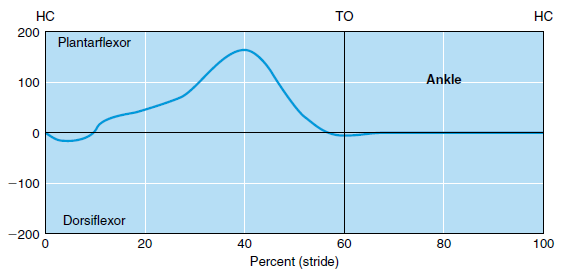
\includegraphics[width=.48\textwidth, keepaspectratio]{fig/id-ankle-ref.png}
%    \end{tabular}
%    \captionof{table}{Σύγκριση εκτιμώμενων ροπών και των αντίστοιχων ροπών με βάση την βιβλιογραφία \cite{whittlesey} για ένα κύκλο βάδισης.}
%    \label{tab:id-hip-knee-ankle-moments}
%\end{center}

%%%%%%%%%%%%%%%%%%%%%%%%%%%%%%%%%%%%%%%%%%%%%%%%%%%%%%%%%%%%%%%%%%%%%%%%%%%%%%%%
\section{Μυϊκή Συσχέτιση}

Στο παρακάτω σχήμα \ref{fig:iber-length-vs-knee-angle} φαίνεται ο τρόπος εκτίμησης του μήκους των μυών μέσα από την γεωμετρική τους τοποθέτηση και η μεταβολή αυτής με την αλλαγή της γωνίας της άρθρωσης δράσεως. Οι δύο μύες ο \eng{rectus femoris} και \eng{vastus intermedius} δρουν στο γόνατο ως καμπτήρες. Ο \eng{rectus femoris} είναι ένας μυς που ξεκινά από την λεκάνη και καταλήγει στην επιγονατίδα, ενώ  ο \eng{vastus intermedius} ξεκινά από την μέση του μηρού και καταλήγει πάλι στην επιγονατίδα. Είναι προφανές ότι όταν το πόδι είναι τεντωμένο τα μήκη των δύο μυών είναι ελάχιστα, ενώ όταν το γόνατο λυγίζει τότε μεγαλώνει το μήκος τους.

\begin{figure}[H]
    \centering
    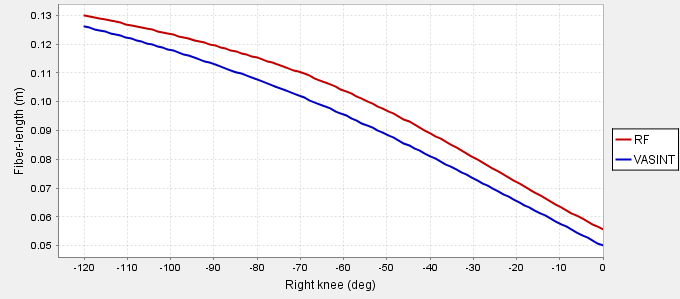
\includegraphics[width=0.8\linewidth, keepaspectratio]{fig/fiber-length-vs-knee-angle.png}
    \caption{Μήκη των δυο μυών του τετρακέφαλου συναρτήσει της γωνίας της άρθρωσης του γονάτου}
    \label{fig:iber-length-vs-knee-angle}
\end{figure}

Στο δεύτερο διάγραμμα \ref{fig:moment-arm-vs-knee-angle} γίνεται μια γεωμετρική ερμηνεία που σχετίζεται με την τοποθέτηση των μυών. Η παράμετρος είναι η ποσότητα που μετατρέπει την δύναμη που παράγει ο μυς σε ροπή στην άρθρωση, η λεγόμενη \eng{muscle moment arm} που αναφέρθηκα στην παράγραφο \ref{subsec:muscle}. Το σημείο ασυνέχειας ($-85^{\circ}$) που παρατηρείται, οφείλεται στο γεγονός ότι για την συγκεκριμένη γωνία οι μύες ξεκινούν να τυλίγονται γύρω από την επιγονατίδα και το μήκος τους διαμερίζεται κατάλληλα με αποτέλεσμα να υπάρχουν ασυνέχειες στους υπολογισμούς.

\begin{figure}[H]
    \centering
    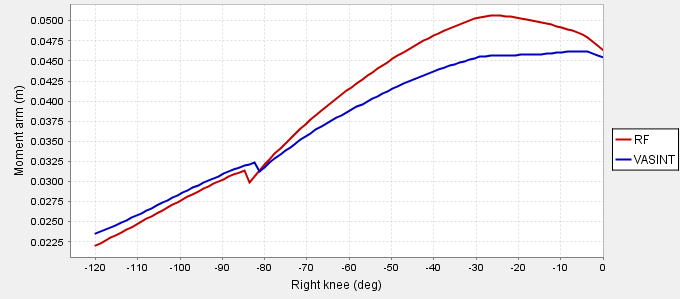
\includegraphics[width=0.8\linewidth, keepaspectratio]{fig/moment-arm-vs-knee-angle.png}
    \caption{Η ποσότητα \eng{moment arm} των δυο μυών του τετρακέφαλου συναρτήσει της γωνίας της άρθρωσης του γονάτου}
    \label{fig:moment-arm-vs-knee-angle}
\end{figure}

Μια άλλη σημαντική ποσότητα είναι η παραγόμενη δύναμη του μυ συναρτήσει της γενικευμένης συντεταγμένης στην άρθρωση. Παρόλο που η μυϊκή δύναμη εξαρτάται και από άλλους παράγοντες μπορεί να γίνει μια ποιοτική αναπαράσταση την κυματομορφής της. Με βάση την θεωρία \ref{subsec:muscle-model} ο μυς έχει ένα παθητικό μέρος που παράγει μια δύναμη όταν αυτός επιμηκύνεται και την παραγόμενη δύναμη που έχει μορφή σαν μια καμπάνα. Όπως φαίνεται στην εικόνα \ref{fig:total-fiber-force}, όπου βλέπουμε το άθροισμα των δυο δυνάμεων, για $-60^{\circ}$ ξεκινά να επιδρά η παθητική δύναμη όσο μικρύνει η γωνία, ενώ για διάστημα $[-60^{\circ},\quad 0^{\circ}]$ έχουμε την καμπάνα παραγωγής δύναμης του μυ.

\begin{figure}[H]
    \centering
    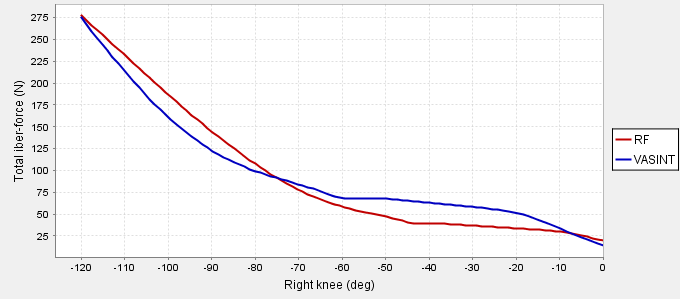
\includegraphics[width=0.8\linewidth, keepaspectratio]{fig/total-fiber-force.png}
    \caption{Η συνολική δύναμη των δυο μυών του τετρακέφαλου συναρτήσει της γωνίας της άρθρωσης του γονάτου}
    \label{fig:total-fiber-force}
\end{figure}

%%%%%%%%%%%%%%%%%%%%%%%%%%%%%%%%%%%%%%%%%%%%%%%%%%%%%%%%%%%%%%%%%%%%%%%%%%%%%%%%
\section{Εκτέλεση Ορθής Δυναμικής}

\begin{figure}[H]
    \centering
    \begin{subfigure}[t]{.48\textwidth}
        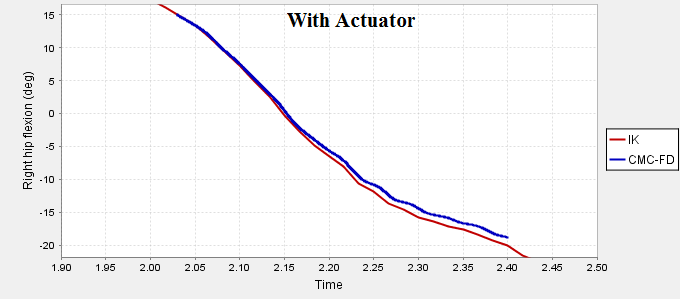
\includegraphics[width=\textwidth, keepaspectratio]{fig/hip-ik-cmc.png}
        \caption{Συντεταγμένη του γοφού}
        \label{fig:hip-cmc}
    \end{subfigure}
    \begin{subfigure}[t]{.48\textwidth}
        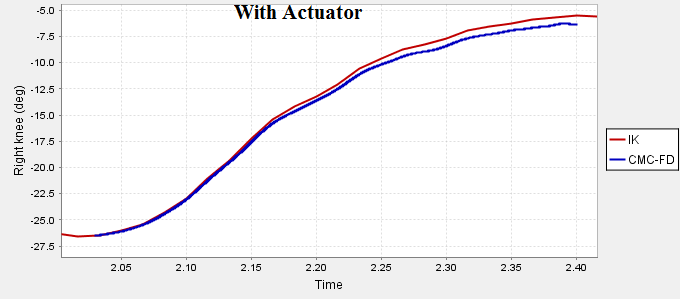
\includegraphics[width=\textwidth, keepaspectratio]{fig/knee-ik-cmc.png}
        \caption{Συντεταγμένη του γονάτου}
        \label{fig:knee-cmc}
    \end{subfigure}

    \centering
    \begin{subfigure}[t]{.48\textwidth}
        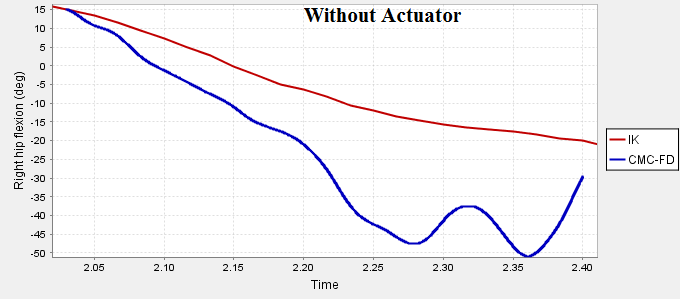
\includegraphics[width=\textwidth, keepaspectratio]{fig/hip-ik-cmc-na.png}
        \caption{Συντεταγμένη του γοφού}
        \label{fig:hip-cmc-na}
    \end{subfigure}
    \begin{subfigure}[t]{.48\textwidth}
        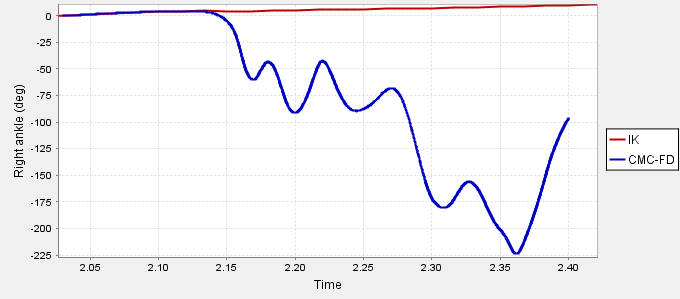
\includegraphics[width=\textwidth, keepaspectratio]{fig/ankle-ik-cmc-na.png}
        \caption{Συντεταγμένη του γονάτου}
        \label{fig:knee-cmc-na}
    \end{subfigure}

    \centering
    \begin{subfigure}[t]{.48\textwidth}
        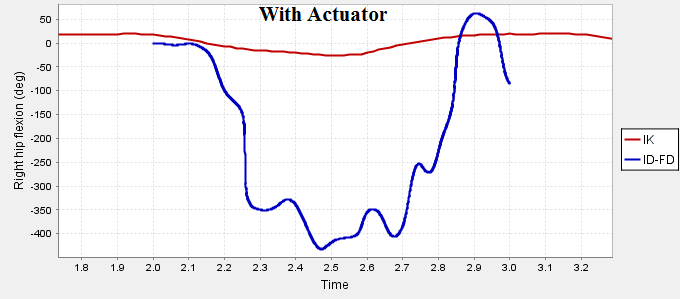
\includegraphics[width=\textwidth, keepaspectratio]{fig/hip-ik-id.png}
        \caption{Συντεταγμένη του γοφού}
        \label{fig:hip-id}
    \end{subfigure}
    \begin{subfigure}[t]{.48\textwidth}
        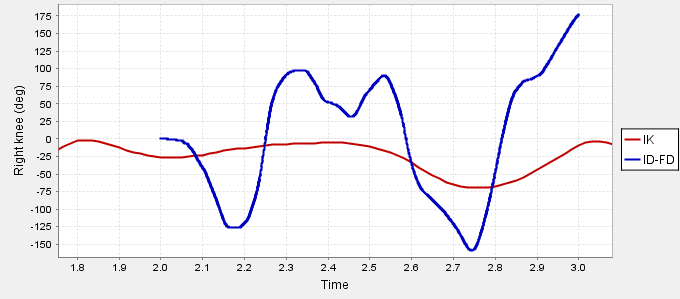
\includegraphics[width=\textwidth, keepaspectratio]{fig/knee-ik-id.png}
        \caption{Συντεταγμένη του γονάτου}
        \label{fig:knee-id}
    \end{subfigure}
    \caption{Σύγκριση της ευστάθειας της ορθής δυναμικής για δυο αρθρώσεις (γοφός, γόνατο). Τροφοδοτούμε την ορθή δυναμική με το αποτέλεσμα της διαδικασία υπολογισμού μυϊκών διεγέρσεων με χρήση εφεδρικών κινητήρων στις αρθρώσεις \ref{fig:hip-cmc}, \ref{fig:knee-cmc}, το ίδιο αλλά χωρίς εφεδρικούς κινητήρες \ref{fig:hip-cmc-na}, \ref{fig:knee-cmc-na} και τέλος συγκρίνουμε με το αν χρησιμοποιήσουμε το αποτέλεσμα της αντίστροφης δυναμικής \ref{fig:hip-id}, \ref{fig:knee-id}}
    \label{fig:fd-cmc-id}
\end{figure}

Σε αυτή την παράγραφο θα αναφερθούμε για την ευστάθεια που επιτυγχάνεται ανάλογα με την κατηγορία μεθόδων που χρησιμοποιούνται. Η ευστάθεια ανταποκρίνεται στη συσσώρευση σφαλμάτων στα στάδια μέχρι τον υπολογισμό των διεγέρσεων, που μπορεί να είναι είτε ροπές, είτε νευρικές διεγέρσεις. Στο πρώτο πείραμα μετά την αντίστροφη κινηματική εκτελούμε την διαδικασία του υπολογισμού των μυϊκών διεγέρσεων \ref{fig:hip-cmc-na}, \ref{fig:knee-cmc-na}, όπου υπολογίζουμε τις διεγέρσεις των μυών που απαιτούνται για την παραγωγή της καταγεγραμμένης κίνησης και κατόπιν εκτελούμε ορθή δυναμική. Πρέπει να αναφέρουμε ότι κατά την διεξαγωγή των πειραμάτων εισάγονται εφεδρικοί κινητήρες \ref{fig:hip-cmc}, \ref{fig:knee-cmc} οι οποίοι είναι σε θέση να τροφοδοτήσουν επιπλέον ροπή στις αρθρώσεις όταν οι μύες δεν είναι σε θέση. Για το λόγο αυτό στα αποτελέσματα γίνεται σύγκριση μεταξύ χρήση ή μη των εφεδρικών κινητήρων. Στο δεύτερο πείραμα μετά την αντίστροφη κινηματική εκτελούμε αντίστροφη δυναμική και τροφοδοτούμε στη συνέχεια τις υπολογισμένες ροπές στην διαδικασία της ορθής δυναμικής ώστε να γίνει σύγκριση \ref{fig:hip-id}, \ref{fig:hip-id}. Στην εικόνα \ref{fig:fd-cmc-id} εξετάζονται οι γενικευμένες συντεταγμένες για τον γοφό και το γόνατο. Με κόκκινο είναι η επιθυμητή τροχιά που θέλουμε να πετύχουμε με βάση το αποτέλεσμα της αντίστροφης κινηματικής ενώ με μπλε το αποτέλεσμα των αναλύσεων. Παρατηρούμε τη μεγάλη σύγκλιση που επιτυγχάνεται με χρήση της μεθόδου υπολογισμού των μυϊκών διεγέρσεων σε συνδυασμό με χρήση εφεδρικών κινητήρων σε σχέση με την αντίστροφη δυναμική, ωστόσο μετά από κάποια χρονική στιγμή η προτεινόμενη μέθοδος μπαίνει και αυτή στην αστάθεια, γεγονός επίσης αναμενόμενο.

%\begin{center}
%    \begin{tabular}{cc}
%        \includegraphics[width=.48\textwidth, keepaspectratio]{fig/hip-ik-cmc.png} & \includegraphics[width=.48\textwidth, keepaspectratio]{fig/knee-ik-cmc.png}\\[3pt]
%        \includegraphics[width=.48\textwidth, keepaspectratio]{fig/hip-ik-cmc-na.png} & \includegraphics[width=.48\textwidth, keepaspectratio]{fig/ankle-ik-cmc-na.png}\\[3pt]
%        \includegraphics[width=.48\textwidth, keepaspectratio]{fig/hip-ik-id.png} & \includegraphics[width=.48\textwidth, keepaspectratio]{fig/knee-ik-id.png}
%    \end{tabular}
%    \captionof{table}{Σύγκριση της ευστάθειας της ορθής δυναμικής}
%    \label{tab:fd-cmc-id}
%\end{center}

Στο σχήμα \ref{fig:rf-vasint-activation} αναφέρεται το αποτέλεσμα των νευρικών διεγέρσεων για τους δυο μύες \eng{rectus femoris} και \eng{vastus intermedius}. Η επιβεβαίωση μπορεί να γίνει ποιοτικά με μετρήσεις από τα \eng{EMG}, ωστόσο δεν έχουμε στην διάθεση μας τέτοιες μετρήσεις.

\begin{figure}[H]
    \centering
    \includegraphics[width=0.8\linewidth, keepaspectratio]{fig/rf-vasint-activation.png}
    \caption{Μυϊκή ενεργοποίηση για τους δυο μύες του τετρακέφαλου}
    \label{fig:rf-vasint-activation}
\end{figure}

%\vfill
%%%%%%%%%%%%%%%%%%%%%%%%%%%%%%%%%%%%%%%%%%%%%%%%%%%%%%%%%%%%%%%%%%%%%%%%%%%%%%%%
\section{Εφαρμογές ή Μελλοντική Εργασία}

Αρχικά θα αναφερθούμε σε συγκεκριμένα σημεία της παρούσας εργασίας που απαιτούν βελτίωση και είναι ενεργό πεδίο έρευνας, ενώ στην συνέχεια θα γίνει μια συζήτηση για πιθανά ενδιαφέρουσες εφαρμογές. Κατά τα στάδια της ανάλυσης έγιναν πολλές προσεγγίσεις που οδηγούν σε εσφαλμένη εκτίμηση της δυναμικής συμπεριφοράς του δείγματος κατά την διεξαγωγή των κινήσεων. 

Ξεκινώντας από το στάδιο της καταγραφής της κίνησης η υλοποίηση που δώσαμε πάσχει από αρκετά προβλήματα που είναι και αναπόφευκτα. Ενδεικτικά δυο σημεία που θα μπορούσαν να βελτιώσουν κατά πολύ το αποτέλεσμα είναι η αντιμετώπιση της παρεμπόδισης και η προσπάθεια καταγραφής πολλαπλών σημείων του σώματος πέραν των αρθρώσεων. Το πρώτο μπορεί να λυθεί αν χρησιμοποιηθούν πολλαπλές συσκευές καταγραφής τοποθετημένες σε διαφορετικές οπτικές γωνίες σε σχέση με το δείγμα, λύνοντας το πρόβλημα της παρεμπόδισης. Όσον αφορά το δεύτερο πρόβλημα θα μπορούσε να υλοποιηθεί καλύτερος αλγόριθμος καταγραφής της κίνησης όπου θα ανιχνεύει περισσότερα σημεία πάνω στο σώμα με αποτέλεσμα να μπορούμε να έχουμε μοναδική λύση στο πρόβλημα της θέσης και του προσανατολισμού των τμημάτων του σώματος. Επαγγελματικά συστήματα καταγραφής ασχολούνται με το πως θα εκτιμήσουν την θέση των ενδείξεων λαμβάνοντας υπόψιν και την κίνηση του δέρματος, όπου είναι τοποθετημένες οι ενδείξεις που ανιχνεύονται. Συμπερασματικά, αντιλαμβανόμαστε την πολυπλοκότητα του προβλήματος και η μείωση του σφάλματος της καταγεγραμμένης κίνησης.

Όσον αφορά το μοντέλο που χρησιμοποιήθηκε έχουν γίνει πολλές προσεγγίσεις. Είναι γνωστό ότι κάθε άνθρωπος έχει τις ιδιαιτερότητες του, τόσο στην δυνατότητα κίνησης όσο και στην γεωμετρία του σκελετού, αλλά και στην γεωμετρία των μυών. Έχουμε εισάγει τρομερές προσεγγίσεις στους βαθμούς ελευθερίας της διάταξής. Για παράδειγμα το γόνατο πέραν της περιστροφικής του ικανότητας εκτελεί και μετατοπίσεις, κάτι που δεν λάβαμε. Τα τελευταία χρόνια γίνεται μια προσπάθεια σάρωσης του δείγμα πριν το πείραμα με μαγνητικό τομογράφο και άλλες συσκευές και με βάση το αποτέλεσμα τους δημιουργείται ένα μοντέλο του σκελετού αλλά και της μυϊκής γεωμετρίας. Όσον αφορά τους μύες με βάση το τελευταίο γίνεται μια προσπάθεια έτσι ώστε ο μυς να μην θεωρείται ένα ευθύγραμμο τμήμα, αλλά να έχει το δικό του όγκο και να αλληλεπιδρά με το γύρω περιβάλλον του. Ωστόσο όλες αυτές οι βελτιώσεις αυξάνουν την πολυπλοκότητα του μοντέλου.

Λόγω της αύξησης της πολυπλοκότητας των μελετούμενων μοντέλων απαιτείται και η αντίστοιχη βελτίωση των μεθόδων που υπάρχουν. Απαιτείται μείωση των σφαλμάτων που εισάγουν, αλλά και η μείωση του χρόνου εκτέλεσης τους. Ειδικά για τον χρόνο εκτέλεσης είναι συχνά καταχρηστικός καθιστώντας την ανάλυση μη κατάλληλη για πραγματικές εφαρμογές.

Ενδιαφέρουσες εφαρμογές θα ήταν η συλλογή αποτελεσμάτων που θα μπορούσαν να βοηθήσουν στους ερευνητές ώστε να κατανοήσουν τα αίτια των ασθενειών με βάση του εικονικού μοντέλου. Επίσης θα μπορούσαν οι τεχνικές που αναπτύχθηκαν στα πλαίσια της παρούσας διπλωματικής εργασίας να χρησιμοποιηθούν στην πράξη δίνοντας άμεσα αποτελέσματα στα αίτια της δυσλειτουργίας της κίνησης χωρίς να χρειαστεί να πάει κανείς στον ιατρό, ενσωματώνοντας συστήματα συμπερασμού που θα κρίνουν με βάση τα αποτελέσματα των αναλύσεων.

Ενδιαφέρον παρουσιάζει και η εφαρμογή τεχνικών προσομοίωσης κατά την παρασκευή φαρμάκων για την θεραπεία του ασθενή. Αν υπήρχαν ακριβή μοντέλα που είναι σε θέση να περιγράψουν με ακρίβεια της λειτουργία του ανθρώπου τότε θα μπορούν αν χρησιμοποιηθούν ώστε να προσομοιάσουν για παράδειγμα το αποτέλεσμα της χορήγησης κάποιου φαρμάκου για την αντιμετώπισης της ασθένειας. Πέραν την προσομοίωση φαρμάκων θα μπορούσε να προσομοιωθεί και το αποτέλεσμα κάποιας εγχείρισης αλλά και να μελετηθεί η ενσωμάτωση για ορθοπεδικών συστημάτων.

Τέλος, κάτι που ανήκει σε διαφορετικό κλάδο, θα ήταν η δημιουργία ενός εικονικού προφίλ του δείγματος, με βάση την φυσιολογία του, κατά την διεξαγωγή κάποιας κίνησης και η εκτίμηση των παραμέτρων που συμβάλουν σε αυτήν. Ως επόμενο στάδιο θα μπορούσε να γίνει η σύνθεση και η δημιουργία διαφορετικών κινήσεων χωρίς να απαιτείται η καταγραφή τους. Επίσης θα μπορούσε να βελτιωθεί το αποτέλεσμα της εικονικής αναπαράστασης της κίνησης λαμβάνοντας υπόψιν πραγματικές παραμέτρους του σώματος, όπως για παράδειγμα η παραμόρφωση των μυών να γίνεται με χρήση της εκτιμώμενης διέγερσης καθιστώντας το πιο ρεαλιστικό.

%%%%%%%%%%%%%%%%%%%%%%%%%%%%%%%%%%%%%%%%%%%%%%%%%%%%%%%%%%%%%%%%%%%%%%%%%%%%%%%%
\section{Συμπεράσματα}

Στην παρούσα εργασία δείξαμε τη δυνατότητα καταγραφής της ανθρώπινης κίνησης με μια φθηνή συσκευή (συγκριτικά με άλλα συστήματα καταγραφής) όπως είναι το \eng{Kinect} για την επίτευξη αξιόλογων αποτελεσμάτων με ελάχιστο κόπο από την πλευρά του προγραμματιστή. Επιπλέον δείξαμε πώς με απλές μεθόδους φιλτραρίσματος μπορεί να βελτιωθεί κατά πολύ το αποτέλεσμα της καταγεγραμμένης κίνησης, ώστε να είναι κατάλληλο για επεξεργασία στα μετέπειτα στάδια. Επίσης κατέστη σαφής η δυνατότητα του \eng{Kinect} να προσδιορίζει τα μορφομετρικά χαρακτηριστικά του ανθρώπου με μεγάλη ακρίβεια.

Στην συνέχεια αποδείξαμε ότι μαζί με την καταγεγραμμένη κίνηση και ένα αξιόπιστο μοντέλο μπορούν να γίνουν πολλές και διάφορες αναλύσεις, που είναι σε θέση να βοηθήσουν τους αναλυτές να εξάγουν συμπεράσματα για το δείγμα. Ως εκ τούτου, απαραίτητο στάδιο της ανάλυσης είναι η αντίστροφη κινηματική, ενώ η μείωση των σφαλμάτων είναι κομβικό σημείο στην ανάλυση. Τονίσαμε την σημασία της αντίστροφης δυναμικής ως εργαλείο ανάλυσης και παρουσιάσαμε τα αποτελέσματα της βάδισης τα οποία συμφωνούν με τη βιβλιογραφία. Παρουσιάσαμε τα αποτέλεσμα της μεθοδολογίας παραγωγής μεγαλύτερης διάρκειας ευσταθούς βάδισης που συμβάδιζαν με μικρή απόκλιση από την επιθυμητή κίνηση. Στα πλαίσια των αναλύσεων μπορούν να εξαχθούν και άλλα αποτελέσματα, όπως είναι οι νευρικές διεγέρσεις, οι δυνάμεις που ασκούν οι μύες, τα μήκη τους κατά την βάδιση και δυνάμεις αντίδρασης μεταξύ των οστών, ωστόσο η πειραματική τους επιβεβαίωση είναι δύσκολη στην πράξη.

Κατά την περιγραφή των μεθόδων ανάλυσης έγιναν συγκρίσεις και αναφέρθηκαν τα μειονεκτήματα και τα πλεονεκτήματα τους. Κατά την σχεδίαση του μοντέλου έγιναν κάποιες παραδοχές που αφορούσαν στην κινητικότητα του, την γεωμετρία των μυών και την κατανομή της μάζας. Όλα αυτά οδηγούν σε σφάλματα στις εκτιμώμενες ποσότητες και ανάλογα με τις ανοχές που έχουμε θέσει με βάση το πρόβλημα ίσως απαιτείται εναλλακτική προσέγγιση. Ωστόσο οι προσεγγίσεις που υιοθετήσαμε οδηγούν σε ορθά αποτελέσματα με μικρές αποκλίσεις από την πραγματικότητα.

Υπάρχει μεγάλο περιθώριο βελτίωσης για την εφεύρεση νέων, πιο γρήγορων, πιο ακριβών μεθόδων. Ειδικά το θέμα του χρόνου που απαιτούν κάποιες αναλύσεις είναι απαγορευτικό πολλές φορές, αλλά και αναπόφευκτο για ένα τόσο δύσκολο πρόβλημα. Η πρόοδος των μεθόδων προσομοίωσης σε συνδυασμό με συστήματα καταγραφής και μεθόδους ανάλυσης μπορούν να χρησιμοποιηθούν στην ιατρική και σε άλλους κλάδους και να γίνουν δεδομένα εργαλεία στην καθημερινότητα, βελτιώνοντας την ποιότητα των υπηρεσιών.
